% In traditional market, the buyer of a swaption has the chance to deposit the principal just before she exercises her option. 
% To create an arbitrage made of a chain of swaptions, the arbitrage buyer needs to buy all the swaptions on the chain and then exercise them simultaneously. For this to happen, the buyer needs to use the late deposit feature that was just mentioned.
% \begin{figure}[H]
%     \centering
%     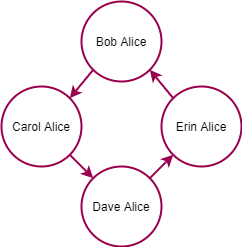
\includegraphics[width=0.5\textwidth]{figures/arb.png}
%     \caption{A loop of swaptions can form an arbitrage.}
%     \label{fig:arbitrage}
% \end{figure}
% To add this feature to the swaptions, we committed some modifications to the original swaption. For the seller to be convinced to deposit his money while the buyer has not deposited yet, the seller can put a secret -let's call it K1- on his money and only under the condition that he sees the same secret on the buyer's principal. Now imagine the next seller in the arbitrage chain -Carol in figure 1. in swaption 2, Alice has to deposit early because she has Bob's final transaction and it contains the secret K1 -if Carol deposits earlier, she puts a new K1. So, Carol will put K1 on her money so that the exchange can only happen if K1 is revealed and Alice can not take Carol's money unless Carol can take hers. Therefore, all the principal deposit transactions in the arbitrage are dependent on revealing of K1. 

% In addition to K1, there is another secret, let's call it A2. This secret is the one that gives buyer the option to exercise the whole swaption or not.

% In order to give Alice the ability to deposit late and Bob the ability to put a secret on his Bcoins, the structure of swaption needs to be modified. Also, the first swaption has to be different from other swaptions in the loop, because only the first one uses the late deposition ability and only in the first swaption one can put a secret on the money and the rest of the swaptions use the same secret.
% So, there would be two types of swpations: 
% \begin{itemize}
%     \item Late-deposit swaption, which comes in the beginning
%     \item Early-deposit swaption, which comes every where else.
% \end{itemize}

% Using the structure in the figure 1, gives us the late deposit ability but it can be too costly for Alice. Since she has to pay margin in every single swaption and she has to generate a lot of transactions and thus transaction fees, she may have to spend more than she originally owns. To Solve that we use another structure for the arbitrage, shown in figure 2.
% \begin{figure}[H]
%     \centering
%     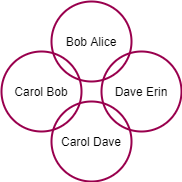
\includegraphics[width = 0.5 \textwidth]{figures/overlapping_arb.png}
%     \caption{arbitrage using overlapping swaptions}
%     \label{fig:arbitrage-overlap}
% \end{figure}

% \subsection{late-deposit swaption}
% figure 3 shows the first type of swaptions. This swaption is the first swaption that Alice creates. Consider the example that was previously mentioned. Bob is the first party Alice trades with and Erin is the last. So, the left blue box of this swaption is shared between Alice and Bob and the right blue box is shared between Alice and Erin.
% Alice is the buyer of swaption, so she pays premium and Bob sells her the option.
% Blue-bordered transactions are broadcast by Bob, pink-bordered ones by Alice and green-bordered ones by Carol. The secret that Bob puts on his money is called K1 and he only reveals it when he sees the same secret on Alice's deposit. In addition, A2 is the secret that gives Alice her option .i.e after K1 is revealed Alice can choose if she wants the arbitrage to exercise or not. If she does not want, she does not reveal A2 otherwise she does. 

% \subsection{early-deposit swaption}
% figure 4 shows the second type of swaptions. This is the type that rest of swaptions are from. The right blue box of this swaption is shared with the left blue box of the previous swaption. Similar to the last one, in this swaption Alice is the buyer and pays the premium but margin and principal are paid by Bob. The left blue box of this swpation is also shared with the right blue box of the next swaption where Dave is the seller of the swaption. purple-bordered transactions are broadcast by Dave. Carol puts the secrets K1 and A2 that she sees on the depositions on her own principal.


% The modified swaptions are in two types: 
% \begin{itemize}
%     \item Late-deposit swaption
% This is the swaption that that lies in the beginning of arbitrage. The buyer is allowed to deposit later than the seller and can deposit just before exercise. It is shown in figure 2. 
% \begin{figure*}
%     \centering
%     \includegraphics[width=0.8\textwidth]{figures/late_swap.png}
%     \caption{Late-deposit swaption, Pink-bordered transactions are broadcast by Alice, blue-bordered ones by Bob, green-bordered ones by Carol}
%     \label{fig:swaption-late-deposition}
% \end{figure*}
% Transactions in the left blue box are common between first and second swaption of the arbitrage.i.e they constitute left part f first swaption and right part of second swaption. So, the right side of this swaption is also shared with the left side of the last swaption.
% So each seller can verify if the parent transactions of the buyer's anyonecanpay transaction are locked with K1 and nothing else. Bob's incentive is the premium. If Alice has not deposited her principal after M time, Bob broadcasts the orange transaction and takes her margin. He also broadcasts the purple transaction and takes his own money. If Alice pays the anyonecanpay transaction, Bob has to reveal K1 because otherwise he will lose his margin and gets nothing(purple transaction has to change a little bit). After K1 is revealed, It's Alice's turn to use her option and reveal A2 or not as she prefers to make the most profit. the delegation part is explained later.
%     \item Early-deposit swaption 
% All other swaptions in an arbitrage are of this kind. In this type unlike the previous one, the buyer deposits earlier than the seller and the buyer is the one who reveals both K1 and A2. It is shown in figure 3.
% \begin{figure*}
%     \centering
%     \includegraphics[width= 0.8\textwidth]{figures/early_swap.png}
%     \caption{Early-deposit swaption, Pink-bordered transactions are broadcast by Alice, blue-bordered ones by Bob, green-bordered ones by Carol, purple-bordered ones by Dave}
%     \label{fig:swaption-early-deposition}
% \end{figure*}
%\end{itemize}

% \subsection{Arbitrage: all swaptions}
% As mentioned before, by putting $n$ swpations, a late-deposit swaption and $n - 1$ early-deposit swaptions next to each other and share the left side of each one with the right side of the one next to it, we can form an arbitrage. The upper part of swaptions (before principal deposit) are created in parallel and the lower parts which take $E+P$ time are concurrent which results in worse case of $M + n + E + n + P + n$ total time, while $n$ sequential swaptions will take $n(M + E + P)$ time.

%$M \leq time \leq M + n(E+\epsilon)$.
% In loop-shaped arbitrages, the input of the buyer's anyonecanpay transaction in the first swaption comes from the last transaction of the last swaption which has the lock of A2 on its output. So, the first swaption's principal deposit cannot be broadcast before A2 is revealed. In line-shaped arbitrage, A2 secret has to be on the principal, so that the option is given to Alice. In this arbitrages, the input of the first swaption's pricipal deposit has to come from a flash loan -not yet implemented in bitcoin. An issue in the loop-shaped one is that Alice cannot extract her final profit. Consider that in each swaption we assume Alice does not take any of the output money and puts all of it in the next swaption which is reasonable because the amounts of money in each swaption is not matter of concern and the ratio is important. Of course if the amount of money is too high this would not be true.

% In both architectures, Alice's signature can be removed from the highlighted blue box, because it is redundant and removing it does not make any harm to the rest of the process(explain more).
% In the figure 4 you can see an arbitrage. The first swaption of the arbitrage, the signatures of Alice and Bob and Dave are needed and in the rest of them only signatures of two participants of the swaption are needed. 

% \begin{figure*}[H]
%     \centering
%     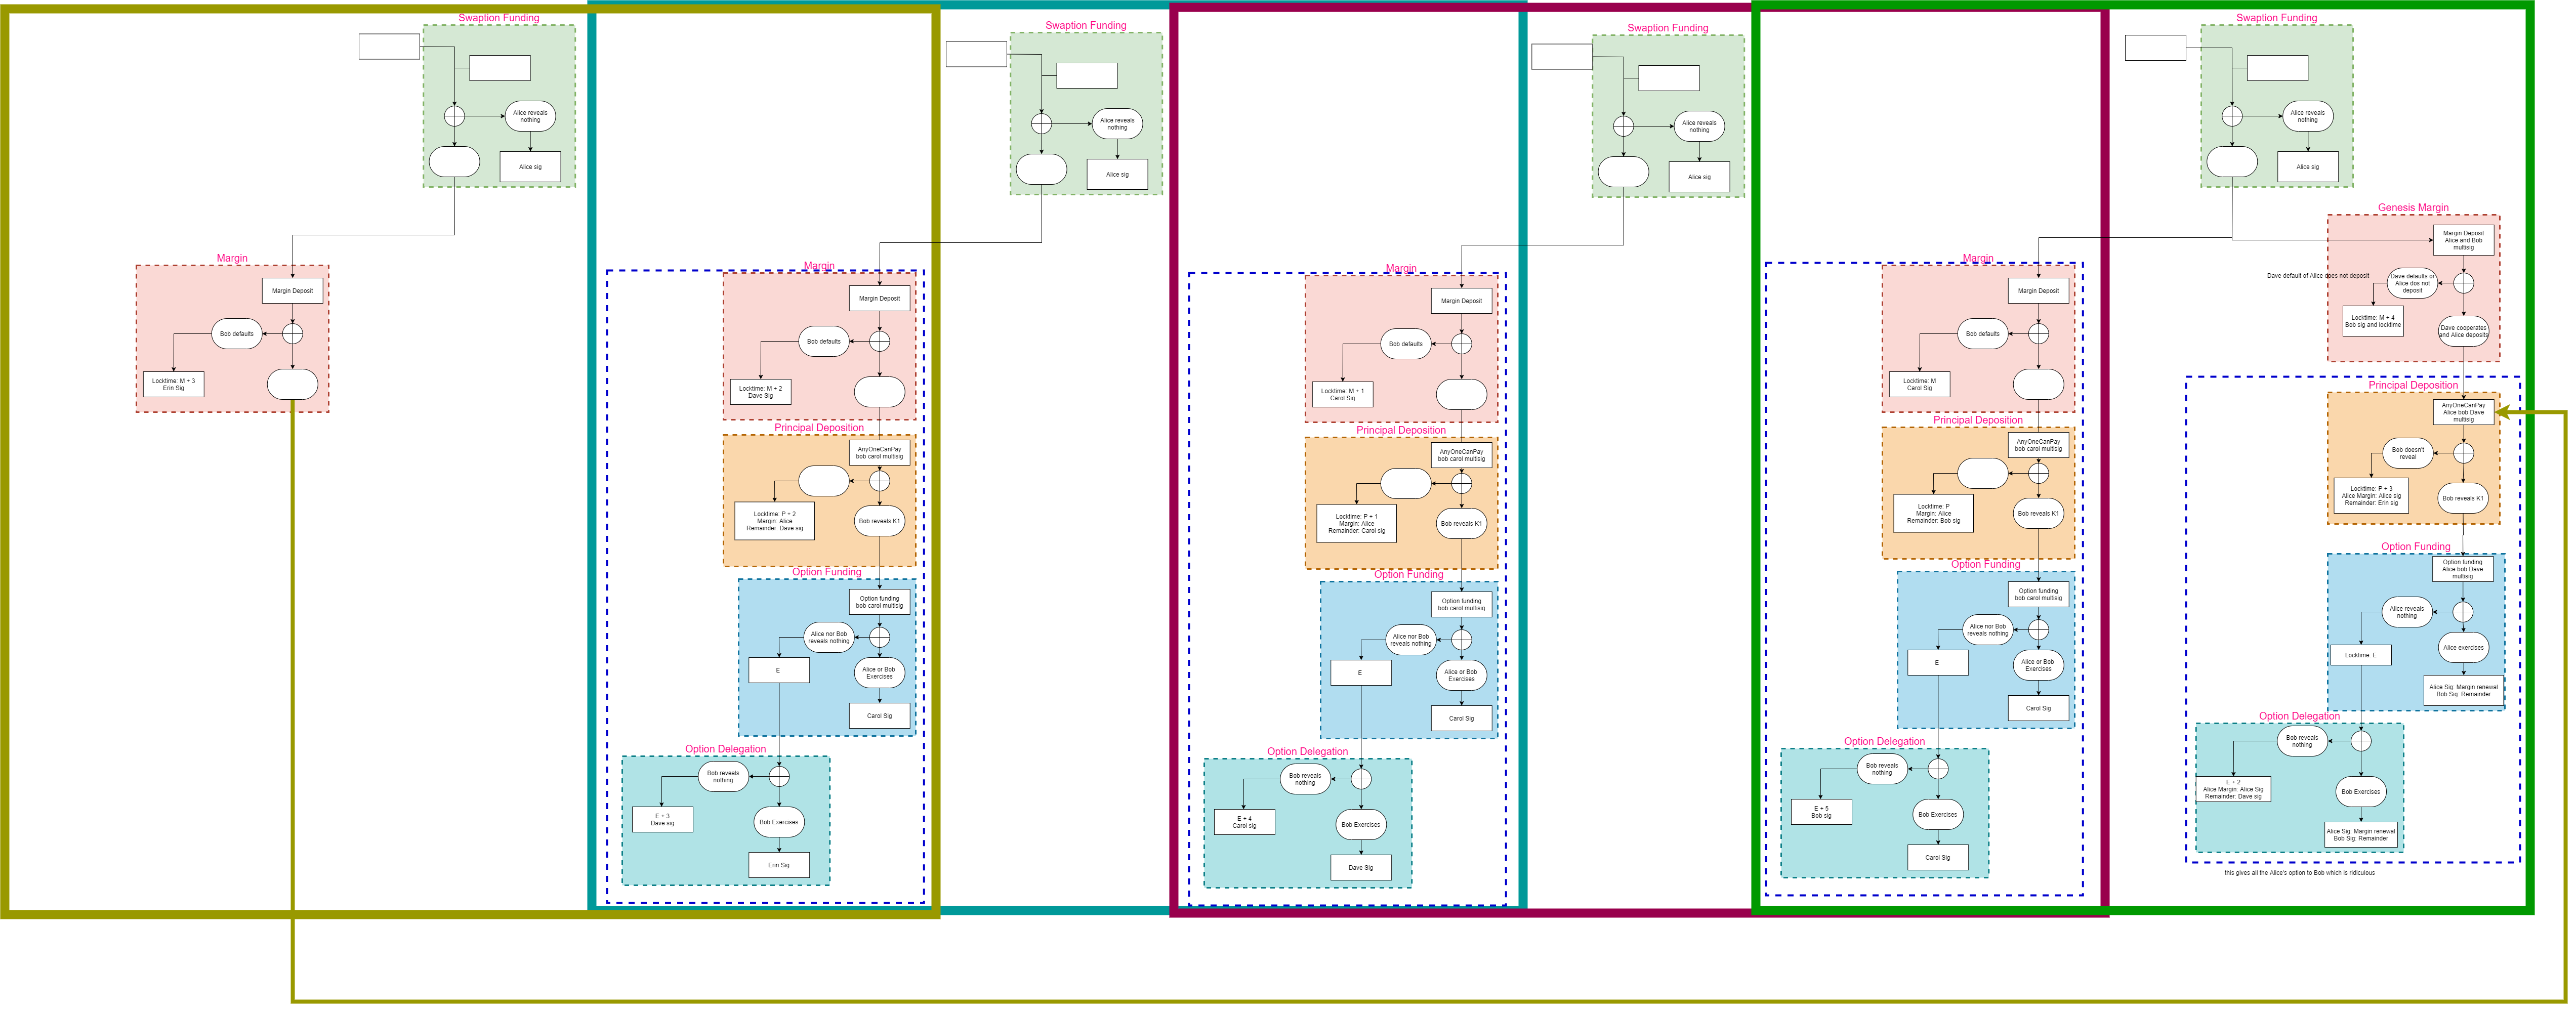
\includegraphics[width = \textwidth]{sections/new_arb.png}
%     \caption{arbitrage}
%     \label{fig:my_label}
% \end{figure*}
% In fist swaption the right side margin deposit timelock has to be bigger than the left side. In the rest of swaptions it is vice versa. So there would be no loop. So is for timelock of the K1 revealing. But in the E part, where Alice wants to reveal A2, in each swaption the the right side timelock has to be bigger than the lest side, so there would be a loop. To solve this problem we add the delegation part to the swaption so that if Alice does not exercise till E, the option is delegated to Bob.


% Figure 5 shows an arbitrage. In this section we explain the procedure in details.
% All transactions are exchanged and signed before anything going on chain. During this not-yet-confirmed transactions sharing, all parties are assured that no one can steal their money. 
% An arbitrage has consists of at least two swaptions. so there are at least three participants: Alice, Bob and Carol. In a typical arbitrage with two exchanges, Alice exchanges her Acoins for Bcoins and then the Bcoins for Acoins. If we put two regular swapitons next to each other, Alice needs to finish the first one and take the Bcoins from Bob to the swaption with Carol which exchanges Bcoin for Acoin and then take the Acoins from Carol to put them in the principal sepoist of the first swaption. This is impossible because the Bob's Acoins can not be taken by Alice unless she has deposited her principal first. However, she can not do that without having swaption with Carol done. Since she can not travel in time this whole process is impossible. Thus, to solve the problem of arbitrage, we need to find a way to let Alice deposit her first swaption's principal late enough so that she can have the outcome of the last swaption and feed it into the first swapiton. Imagine we solve this problem. %todo: fill this shit
% There would be other considerations. First, what would be Bob's incentive to reveal the secret? Secondly, how would be the timelocks? how would each person make sure she would be safe? and ...

% even if all the problems are solved and swaptions are put next to each other, so Alice has to put margin for every single one of them, this would cost a lot for her if she defaults, and this will reduce her option. 
%todo: not sure

% To solve that we design the arbitrage such that swaptions can overlap and Bob's margin and principal directly goes to Carol's, with no need for Alice to meddle. This way, number of total transactions is almost half and Alice only pays one margin. 
% Now the detailed process of the arbitrage is discussed. 

% \begin{enumerate}
%     \item Alice and Bob exchange funding transactions with HTLC and A1 secret. Alice also does that with every other 
% swaption's other party.
%     \item they exchange refund transactions in case Alice does not reveal A1
%     \item all the transactions are exchanged.
%     \item if Alice does reveal A1, the margin deposit transactions go on chain
%     \item Alice has a time of M + 4 blocks to deposit her principal, while Bob has M blocks for that. Alice's  principal 
% contains her margin and Erin's margin. So in case of canceling the arbitrage, Alice and Erin will both take back their margin
% from the output of Alice's principal deposition transaction.
%  if Alice does not deposit until M + 4 blocks, Bob takes her margin. if Bob does not deposit his principal, till 
% M blocks, Carol will take his principal, because Bob and Carol are the two parties of the second swaption.
% if Bob does not deposit, Carol takes his margin and she herself will not deposit her principal, so Dave takes her 
% margin and does not deposit, so Erin takes her margin and does not deposit, 
% so Alice takes her margin and does not deposit, so Bob takes her margin and every thing ends. So, the locktimes
% for the principal depositions have to have an ascending order. Bob have M blocks, Carol M + 1, Dave M + 2, Erin 
% M + 3 and Alice M + 4. In addition, if Bob deposits within M blocks and Alice does not till M + 4, Bob takes her margin
% and does not reveal K1.
%     \item if Bob and Alice and every other party deposit their principals, we go to the next stage --the orange boxes. In this stage Bob has a 
% time of P blocks, which is relatively short, to reveal K1. revealing K1 means that Bob puts the next transaction, the 
% so-called option funding transaction. Carol also has P + 1 blocks time to put the option funding transaction and so reveal 
% K1 for Dave and this goes on to the last party in the arbitrage chain. meanwhile Alice has the time of P + 4 block time to put 
% her option funding transaction on chain. If Bob does not reveal K1, Alice puts the default transaction on chain and 
% takes Bob's margin while returning the rest of his principal to him.  Carol also puts the default transaction on chain
% and takes her own principal back. this goes on to the last swaption. only the last one, Erin, gets her payback 
% slightly differently. Hence Alice's principal contains both her margin and Erin's margin
%  in the case of K1 not being revealed, Alice gets her margin back and Erin gets the rest. So if Bob defaults, 
% everyone gets their money back and Bob himself looses his margin. So, Bob does not have incentive 
% to default at this stage(what if Acoin is much more than Bcoin in value?). On the other hand, if 
% Bob reveals K1 .i.e put the option funding transaction on chain, every other participant including Alice will put their option
% funding transaction on chain. 
%     \item Funding transactions have Alice's option secret, A2, on its output, so finally gives Alice her option she has paid premium for.
% In this stage, because Alice has to reveal, she her locktime needs to be more than Bob's. So if for the rest
% of the loop .i.e Bob's locktime has to be longer than Carol's. Carol's longer than Dave's and Dave's longer than 
% Erin's and Erin's longer than Alice. which is impossible. so we solve this problem by adding the delegation stage.
% Imagine the locktimes are so: Bob E + 5, Carol E + 4, Dave E + 3, Erin E + 2 and Alice E + 1. In this 
% situation, Bob can not trust Alice and if Alice is rational she will definitely steal Bob's money. Here comes the 
% delegation part. 
%     \item To convince Bob to participate, Alice promises she will reveal A2 within E blocks, otherwise
% delegates her option to Bob. So in each swaption if Alice does not reveal A2 until E blocks, Bob and every other
% party puts on chain. from now on Bob owns the option. In this stage Bob will not exercise because if the whole
% arbitrage was beneficial Alice would have done it (why?) and so he lets every thing to cancel and all the money 
% go back to their original owner. So technically, Alice still owns the option because if she defaults Bob also defaults.
% On the other hand, the probability of Alice default is so low because this is an arbitrage and arbitrages are
% with a high probability beneficial (according to the definition)(forgot the exact word, check it).
% \end{enumerate}
% note that there are five participants, four common parts but five margin deposits. the reason is that every party has to pay the margin so that there is a way to punish them if they defaulted. Alice needs to put her margin even though Erin puts margin, to prove to Bob that she would not steal his margin. 

% in every cancelation transaction in the first swaption Alice takes her margin back, so after she deposits her principal, she will definitely take her margin back. In other swaptions get back to their owners in case of canceling as they are already in the principal. In the first swaption, Alice's margin is kinda added to the principal. 

% note that the option funding has two signatures on it in every where except the first swaption where it had three signatures. the reason is it contains Alice, Bob and Erin's money so it needs their signatures.

% note that Alice only deposits when every thing has gone well in all the swpations i.e. every one has deposited their principal. otherwise if she deposits before every one had deposited, after revealing of K1, the not-yet-deposited party will take Alice's principal without paying his principal. If Alice deposits her principal, Bob definitely reveals K1. So, looking carefully the rest of the transactions are not needed.
% \subsection{Arbitrage: loan plus swpations}
% This is a type of arbitrage in which the arbitrage owner starts with a non-collateralized loan and uses her borrowed money in some swaptions and then gives her debt back.

% In economics and finance, arbitrage is the practice of taking advantage of a price difference between two or more markets: striking a combination of matching deals that capitalize upon the imbalance, the profit being the difference between the market prices at which the unit is traded.

% Arbitrage occurs when an investor can make a profit from simultaneously buying and selling a commodity in two different markets.

% The simultaneous chains of buying and selling various securities  two different markets, resulting in profits without risk. Perfectly efficient markets present no arbitrage opportunities. Perfectly efficient markets seldom exist, but, arbitrage opportunities are often precluded because of transactions costs.